\documentclass[conference]{IEEEtran}
\usepackage{cite}
\usepackage{amsmath,amssymb,amsfonts}
\usepackage{algorithmic}
\usepackage{algorithm}
\usepackage{graphicx}
\usepackage{textcomp}
\usepackage{xcolor}
\usepackage{booktabs}
\usepackage{multirow}
\usepackage{hyperref}
\usepackage{balance}

\newtheorem{theorem}{Theorem}
\newtheorem{corollary}{Corollary}
\newcommand{\rhomax}{\rho_{\max}}

\begin{document}

\title{Predict, Place, Refine: Non-Locality-Guided Express Link Placement for LLM Chiplet Networks}

\author{
\IEEEauthorblockN{Youngwoo Jeong}
}

\maketitle

\begin{abstract}
We argue that a single static workload property---the \textit{non-locality fraction} (NL\%, the share of traffic volume between non-adjacent chiplet pairs)---predicts both how much express links help a chiplet network-on-interposer (NoI) and how much refinement headroom remains after a strong heuristic is applied. Building on this predictor, we organize express-link placement around three steps: \textsc{Predict} with NL\%, \textsc{Place} with a workload-aware greedy allocator, and \textsc{Refine} with warm-start reinforcement learning guarded by a measured BookSim fallback.

We first prove that center-link amplification under adjacent-only routing grows as $\Theta(K^{3/2})$ and that no routing algorithm eliminates this structural tax, motivating express links as a topological rather than allocation-level fix. Across 40 BookSim configurations spanning four LLM workloads, two chiplet counts, two per-chiplet mesh sizes, and multiple link budgets, greedy express placement improves latency by \textbf{25.6\%} on average over adjacent-uniform no-express baselines, and \textbf{RL-WS}---warm-start RL with post-hoc BookSim fallback---raises this to \textbf{28.2\%}. The best single configuration reaches \textbf{56.6\%} latency reduction on MoE Skewed, $K$=32, $N$=8, 4$\times$ budget (multi-seed mean across three independent seeds: $56.57\%\!\pm\!0.55\%$). Pooled across the 40 workload-configuration pairs, NL\% predicts express saving with Spearman $\rho=0.744$ ($p=3.8\times 10^{-8}$) under greedy and RL-WS+fallback alike; restricted to 16 best-budget cells aggregated over three seeds each, $\rho=0.776$ ($p=4.1\times 10^{-4}$). Multi-seed evaluation (48 RL-training runs, three seeds per cell) shows per-cell RL-WS+fallback saving variance $\le 1.22\%$ and activates the fallback on 20.8\% of seed-runs---predominantly on low-NL\% $K{=}16$ cells---turning what would be a $-1.77\%$ worst-case raw-RL regression into a measured zero-regression guarantee. On unseen ring-allreduce, pipeline-parallel, and all-to-all workloads, RL-WS wins 6/6 evaluated cases; a zero-shot GNN baseline is competitive on ring and pipeline but collapses on all-to-all, and per-cell fine-tuning the same GNN does not close the all-to-all gap ($-23.5\%$ mean) because the collapse is architectural rather than training-coverage driven, making RL-WS the robust choice under distribution shift.
\end{abstract}

% ============================================================
\section{Introduction}
% ============================================================

AI accelerator chiplet counts are scaling rapidly: AMD's MI300X integrates 8 compute chiplets~\cite{mi300x}, NVIDIA's B200 connects 2 dies~\cite{blackwell}, and industry roadmaps project 16--64 chiplets in next-generation designs. Each additional chiplet demands inter-chiplet bandwidth provisioned through the Network-on-Interposer (NoI)---typically by adding die-to-die links only between adjacent chiplets on the silicon interposer~\cite{kite,florets,ucie}.

\begin{figure}[t]
\centering
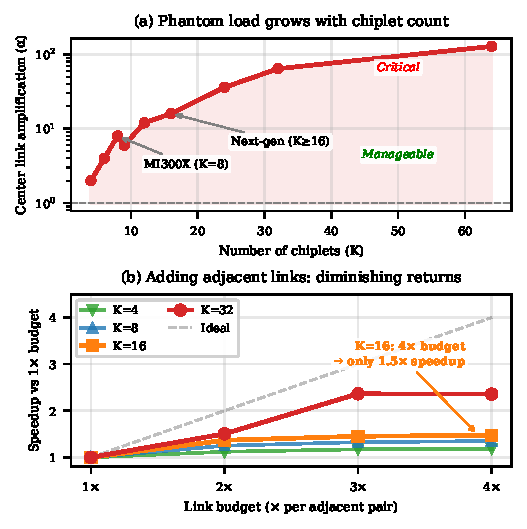
\includegraphics[width=0.95\columnwidth]{figures/fig_intro_motivation.pdf}
\caption{The phantom load problem. (a)~Center-link amplification grows super-linearly with chiplet count. (b)~Adding adjacent links yields diminishing returns: at $K$=16, 4$\times$ budget gives only 1.5$\times$ speedup.}
\label{fig:motivation}
\end{figure}

However, adding adjacent links has sharply diminishing returns (Fig.~\ref{fig:motivation}). In a 2D chiplet grid, non-adjacent traffic must traverse intermediate links via multi-hop routing, creating \textit{phantom load}: intermediate links carry routing traffic far exceeding their direct demand. We prove that center links in a $K$-chiplet square grid carry $\Theta(K^{3/2})$ times more traffic than their direct demand. At $K$=32, this amplification reaches 64$\times$ on center links, forcing designers to provision far more adjacent links than would be needed if traffic could reach its destination directly.

Prior NoI work~\cite{kite,florets} optimizes allocation among adjacent pairs---choosing \textit{which} adjacent links receive more capacity. But phantom load is not merely an allocation problem; it is a topological one. Express links---direct interposer connections between non-adjacent chiplets---attack the root cause by bypassing overloaded intermediate links. Recent learning-based NoI synthesis~\cite{parl} trains reinforcement learning from scratch on a multi-objective interference score, but without a workload-level predictor and without any measured guarantee against a strong heuristic, which leaves placement behavior opaque on out-of-distribution traffic.

This paper organizes express-link placement around three steps: \textsc{Predict}, \textsc{Place}, and \textsc{Refine}. \textsc{Predict} asks whether a workload has enough non-local traffic for express links to matter at all, using NL\% as a single scalar. \textsc{Place} produces a strong deterministic allocation via workload-aware greedy search. \textsc{Refine} improves that allocation with warm-start reinforcement learning and protects against regressions with a measured BookSim fallback. The three steps are complementary: NL\% predicts \textit{both} raw express-link benefit \textit{and} the headroom that remains for RL on top of greedy.

Our contributions map directly onto these three steps:
\begin{itemize}
\item \textbf{C1. Predict: NL\% as a simulation-free predictor.} We define NL\% on the pre-routing demand matrix and show that it predicts measured express-link saving with Spearman $\rho=0.74$ ($p<10^{-7}$) across 40 workload-configuration pairs, letting architects decide whether express links are worth considering from a single static statistic. We complement this with a closed-form $\Theta(K^{3/2})$ phantom-load bound and routing-algorithm independence results that isolate the structural role of non-adjacent traffic.
\item \textbf{C2. Place: Workload-aware greedy with full budget utilization.} We present a greedy express placement algorithm with traffic-proportional budget fallback that always consumes the allocated link budget, including on sparse traffic patterns. Across 40 BookSim configurations, greedy alone obtains a 25.6\% mean latency saving versus an adjacent-uniform no-express baseline, serving as a strong deterministic foundation.
\item \textbf{C3. Refine: Warm-start RL with measured safety.} We introduce RL-WS, a swap-based reinforcement-learning refinement initialized from the greedy solution and followed by a post-hoc BookSim fallback that keeps the lower-latency of \{greedy, RL\}. RL-WS improves the mean saving to 28.2\% (best case 56.4\%), beats greedy in 35/40 configurations, and is never worse than greedy by construction. On six unseen workload-configuration cells (ring-allreduce, pipeline-parallel, all-to-all), RL-WS wins all six; both a zero-shot GNN and a per-cell fine-tuned GNN collapse on all-to-all (mean $-23.5\%$), confirming that the collapse is an architectural limit of edge-scoring GNNs on uniform traffic rather than a training-coverage issue, and that RL-WS is the robust choice under distribution shift.
\end{itemize}

% ============================================================
\section{Background and Related Work}
% ============================================================

\textbf{Adjacent-only NoI design.}
Kite~\cite{kite} and Florets~\cite{florets} optimize adjacent-only chiplet topologies and link allocation. These approaches improve link placement among neighboring chiplets, but they cannot remove the multi-hop structure that creates phantom load in the first place.

\textbf{Express channels in monolithic NoC.}
Express Virtual Channels~\cite{express_vc} and concentrated meshes~\cite{cmesh} bypass intermediate hops within a single die. In monolithic NoCs, wire delay is relatively small and the optimization target is hop count. In chiplet NoI, each inter-chiplet link consumes scarce die-edge PHY area and interposer routing resources, so the main problem is not just latency but the \textit{cost} of transit traffic.

\textbf{Learning-based topology synthesis.}
The closest prior work is PARL~\cite{parl}, which applies cold-start maskable PPO to NoI topology synthesis for mixed DL workloads. PARL optimizes a multi-objective interference score but does not use a workload-level predictor, does not warm-start from a strong heuristic, and offers no worst-case guarantee relative to a deterministic baseline. Our method differs along three orthogonal axes simultaneously: (i) NL\% as a simulation-free \textit{predictor} of both benefit and headroom, (ii) \textit{warm-start} RL initialized from a workload-aware greedy allocator, and (iii) a \textit{post-hoc BookSim fallback} that makes the measured latency never worse than greedy. A direct experimental reproduction of PARL on our 40-configuration benchmark would require re-implementing its multi-objective reward and interference evaluator on BookSim traces; we instead position PARL qualitatively in Table~\ref{tab:related} along the three axes where our design choices diverge, and treat an end-to-end reproduction as future work. The ablation in Section~\ref{subsec:ablation} does include a \textit{cold-start} variant of our own RL, which serves as a best-effort internal proxy for the cold-PPO regime that PARL inhabits: cold RL's worst-case is $+11.3\%$ vs greedy, whereas warm-start's worst-case is $+1.7\%$ before fallback and $+0.0\%$ after fallback.

\begin{table}[t]
\centering
\caption{Comparison with Prior Work Along the Three Novelty Axes (Predictor / Warm-Start / Safety)}
\label{tab:related}
\scriptsize
\begin{tabular}{lcccc}
\toprule
Work & Target & Predictor? & Warm-start? & Safety \\
\midrule
Kite~\cite{kite} & adj.\ topology & No & N/A & -- \\
Florets~\cite{florets} & adj.\ topology & No & N/A & -- \\
PARL~\cite{parl} & NoI synthesis & No & Cold PPO & None \\
\textbf{Ours} & express place. & \textbf{NL\%} & \textbf{Greedy} & $\le$ Greedy \\
\bottomrule
\end{tabular}
\end{table}

% ============================================================
\section{Phantom Load Analysis}
% ============================================================

\subsection{Physical Substrate and Chiplet Grid}

\begin{figure*}[t]
\centering
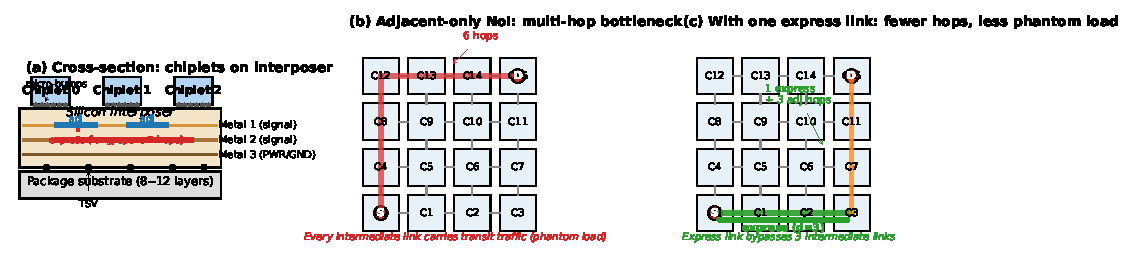
\includegraphics[width=0.98\textwidth]{figures/fig_interposer_structure.pdf}
\caption{Physical substrate and the source of phantom load. (a)~Vertical cross-section: chiplets sit on a silicon interposer that contains a small number of metal routing layers (typically 3--6 in current CoWoS); adjacent links are short horizontal wires while an express link is a longer wire that may traverse vias across layers. (b)~Top-down view of a $4\times 4$ chiplet grid with only adjacent links: communication between corner chiplets S and D requires six hops, and every intermediate link must carry that transit traffic (phantom load). (c)~Adding a single distance-3 express link (green) absorbs three of the intermediate hops in one physical wire, eliminating phantom load on those links. Our paper asks which non-adjacent pairs should receive such express wires under a fixed interposer routing budget.}
\label{fig:interposer}
\end{figure*}

Fig.~\ref{fig:interposer}(a) shows the physical substrate assumed throughout the paper: a \textbf{2.5D chiplet package} in which multiple dies sit side-by-side on a silicon interposer, as realized by TSMC CoWoS-S/L and Intel EMIB. $K$ compute chiplets sit on a silicon interposer; communication between chiplets goes through the interposer's metal routing layers, which in current CoWoS-class packages expose only 3--6 signal layers---an order of magnitude fewer than a server-class PCB. UCIe 1.x and 2.0 D2D PHY specifications~\cite{ucie} are strictly point-to-point, so every inter-chiplet link is a dedicated wire between exactly two chiplets, and no on-interposer switching fabric exists in ratified standards. Combined with reticle-bounded interposer area (currently $\le 2500$\,mm$^2$), the dominant integration paradigm in commercial chiplet products (AMD MI300~\cite{mi300x}, NVIDIA B200~\cite{blackwell}, Apple M-series UltraFusion, Intel Ponte Vecchio) is a mesh-like layout of compute chiplets with point-to-point UCIe/D2D connectivity.

In this paradigm, traffic between non-adjacent chiplets must traverse multiple physical links in sequence. Fig.~\ref{fig:interposer}(b) illustrates the resulting phantom load on a $4\times 4$ grid: a single S$\to$D flow between diagonally opposite chiplets forces six intermediate links to carry transit traffic for which they have no endpoint demand. An \textit{express link}---a long direct wire on an unused routing channel between a pair of non-adjacent chiplets---absorbs several of these hops at once (Fig.~\ref{fig:interposer}(c)). Physically, the express link consumes interposer wire area proportional to its length, may transition between metal layers through vias, and requires a UCIe PHY at each end (one per chiplet beachfront slot). The total interposer wire budget is therefore a scarce, shared resource, and the central question of this paper is: \textit{given a fixed routing budget and a known workload, which non-adjacent pairs should receive an express link?}

\subsection{System Model}

We consider $K$ chiplets arranged on an $R \times C$ 2D grid on a silicon interposer (e.g., $K$=16 in a 4$\times$4 grid). Each chiplet pair $(i,j)$ has traffic demand $T[i,j]$ (GB/s). In conventional NoI, links connect only \textit{adjacent} pairs---chiplets at Manhattan distance 1. When chiplet $i$ communicates with non-adjacent chiplet $j$, the traffic must traverse a multi-hop path through intermediate chiplets.

The \textit{load} on an adjacent link $(a,b)$ is the total traffic from \textit{all} flows whose routing path crosses it:
\begin{equation}
\text{Load}(a,b) = \sum_{\substack{(i,j): \text{path}(i,j) \\ \text{crosses } (a,b)}} T[i,j].
\end{equation}

We define the \textit{amplification factor}
\begin{equation}
\alpha(a,b) = \frac{\text{Load}(a,b)}{T_{\text{direct}}(a,b)},
\end{equation}
where $T_{\text{direct}}(a,b)$ is the traffic directly exchanged by chiplets $a$ and $b$. Large $\alpha$ indicates that the link is dominated by phantom load rather than its own endpoint demand. Fig.~\ref{fig:phantom4x4} concretizes this on a 4$\times$4 grid: a single long-distance flow C0$\to$C15 traverses six adjacent links, five of which are pure transit; adding one express link at distance $d=3$ bypasses two of those transit links at once.

\begin{figure}[t]
\centering
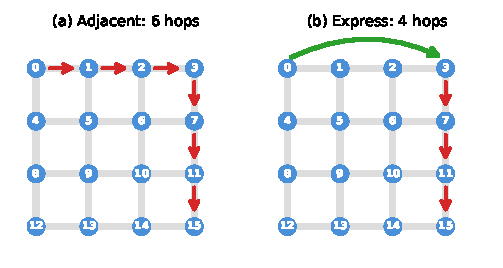
\includegraphics[width=0.95\columnwidth]{figures/fig_phantom_4x4.pdf}
\caption{Phantom load example on a 4$\times$4 chiplet grid. (a)~Adjacent-only: C0$\to$C15 requires 6 hops via XY routing; every intermediate link carries transit traffic. (b)~An express link C0$\to$C3 reduces the path to 4 hops, freeing 2 intermediate links.}
\label{fig:phantom4x4}
\end{figure}

\subsection{Closed-Form Scaling}

We derive an exact formula for the number of flows crossing each link under XY routing with uniform all-to-all traffic.

\begin{theorem}[Flow count at link boundaries]
Under XY routing with uniform all-to-all traffic on an $R \times C$ grid, the number of directed flows crossing each link is
\begin{align}
F_H(c) &= 2R \cdot (c{+}1)(C{-}c{-}1), \\
F_V(r) &= 2C \cdot (r{+}1)(R{-}r{-}1),
\end{align}
for a horizontal boundary at column $c|c{+}1$ and a vertical boundary at row $r|r{+}1$, respectively.
Since each adjacent pair contributes exactly 2 direct flows, the center-link amplification factor satisfies
\begin{equation}
\alpha_{\max} \;=\; R \cdot \lceil C/2 \rceil \cdot \lfloor C/2 \rfloor.
\end{equation}
\end{theorem}

\begin{corollary}[$\Theta(K^{3/2})$ scaling for square grids]
\label{cor:theta}
For square grids with $R=C=\sqrt{K}$, $\alpha_{\max} = \sqrt{K} \cdot \lfloor K/4 \rfloor = \Theta(K^{3/2})$; center-link amplification therefore grows super-linearly with chiplet count.
\end{corollary}

\textbf{Example.} On a 4$\times$4 grid, the center horizontal link at $c$=1 carries $F_H(1) = 2 \times 4 \times 2 \times 2 = 32$ directed flows, and since each adjacent pair contributes only 2 direct flows, amplification is $\alpha = 32/2 = 16\times$. Table~\ref{tab:scaling} validates Corollary~\ref{cor:theta} across grid sizes up to $K$=64.

\begin{table}[t]
\centering
\caption{Phantom Load Scaling Across Grid Sizes}
\label{tab:scaling}
\footnotesize
\begin{tabular}{lcrrrr}
\toprule
Grid & K & Max $\alpha$ & Avg $\alpha$ & P95 $\alpha$ & Imbalance \\
\midrule
2$\times$2 & 4 & 2 & 2.0 & 2.0 & 1.0 \\
2$\times$4 & 8 & 8 & 5.6 & 8.0 & 2.0 \\
4$\times$4 & 16 & 16 & 13.3 & 16.0 & 1.3 \\
4$\times$8 & 32 & 64 & 38.2 & 64.0 & 2.7 \\
8$\times$8 & 64 & 128 & 96.0 & 128.0 & 2.3 \\
\bottomrule
\end{tabular}
\end{table}

\textbf{Why this is a cost problem.} To keep the most congested link below utilization target $\rho^*$, an adjacent-only topology must provision $\lceil \alpha_{\max} / \rho^* \rceil$ links on center pairs. At $K$=64, this implies over two orders of magnitude more capacity than direct demand alone would require.

\subsection{Routing Algorithm Independence}

A natural question is whether smarter routing eliminates phantom load. Table~\ref{tab:routing} compares XY/YX, ECMP, and Valiant routing. The values below are simulator-measured \textit{directional} link loads and therefore are not directly comparable to the undirected closed-form values in Table~\ref{tab:scaling}; the point is comparative, not absolute.

\begin{table}[t]
\centering
\caption{Load Imbalance Across Routing Algorithms}
\label{tab:routing}
\footnotesize
\begin{tabular}{llrr}
\toprule
Grid & Routing & Max $\alpha$ & Imbalance \\
\midrule
\multirow{4}{*}{4$\times$4} & XY & 111 & 8.2 \\
& YX & 223 & 8.2 \\
& ECMP & 94 & 2.3 \\
& Valiant & 347 & 3.1 \\
\midrule
\multirow{4}{*}{4$\times$8} & XY & 123 & 18.7 \\
& YX & 246 & 18.7 \\
& ECMP & 234 & 6.1 \\
& Valiant & 417 & 5.2 \\
\bottomrule
\end{tabular}
\end{table}

ECMP distributes load more evenly than XY/YX, but the center links still lie on more shortest paths and remain over-utilized. Valiant further smooths imbalance but doubles total path length. Phantom load is therefore a structural consequence of multi-hop adjacency, not an artifact of one routing algorithm.

% ============================================================
\section{Non-Locality Analysis}
% ============================================================

We define the \textit{non-locality fraction} on demand matrix $T$ and chiplet graph $G$ as
\begin{equation}
\mathrm{NL\%}(T,G) =
\frac{\sum_{i<j:\,\mathrm{hop}_G(i,j)\ge 2} \left(T[i,j] + T[j,i]\right)}
{\sum_{i<j} \left(T[i,j] + T[j,i]\right)}.
\end{equation}
NL\% is computed on the pre-routing demand matrix. It is therefore a static workload property relative to a chosen chiplet layout and lets us predict whether non-adjacent shortcuts are even worth considering before simulation.

\textbf{NL\% predicts measured saving.}
Empirically, NL\% correlates strongly with express-link saving across the full evaluation set. Pooling all 40 workload-configuration pairs (4 workloads $\times$ $\{K\!=\!16,32\}$ $\times$ $\{N\!=\!4,8\}$ $\times$ 2--3 budget levels), the Spearman rank correlation between NL\% and greedy-express saving versus adjacent-uniform is $\rho=0.744$ ($p=3.8\times 10^{-8}$), and the ties-robust Kendall correlation is $\tau=0.593$ ($p=9.6\times 10^{-7}$). The correlation is stable under refinement: replacing greedy by warm-start RL with fallback yields $\rho=0.744$ ($\tau=0.596$). Restricted to 16 best-budget cells (one per workload-$K$-$N$), the correlations are $\rho=0.740$ ($\tau=0.615$) for greedy and $\rho=0.764$ ($\tau=0.634$) for RL-WS+fallback on single-seed data; aggregating the same 16 cells across three independent RL-WS seeds raises the correlation slightly to $\rho=0.776$ ($\tau=0.652$, $p=4.1\times 10^{-4}$), indicating that the NL\%$\to$saving ordering is robust to stochastic RL variance. Because our four training workloads occupy four distinct NL\% tiers, we report $\tau$ alongside $\rho$ to confirm that the monotone trend is not an artifact of tie-breaking in the rank correlation. The same NL\% ordering also predicts the RL headroom over greedy (Section~\ref{subsec:main}), so a single static statistic lets architects both \textit{screen} workloads for express investment and \textit{decide} whether to invoke RL refinement on top.

We evaluate four representative chiplet communication patterns at $K$=32. These form the training workloads for the learned placement methods; ring-allreduce, pipeline-parallel, and all-to-all are revisited later as unseen generalization workloads.

\begin{table}[t]
\centering
\caption{LLM Workloads and Non-Locality ($K$=32)}
\label{tab:workloads}
\scriptsize
\begin{tabular}{lrrrrl}
\toprule
Workload & NL\% & Max $\alpha$ & Imbal. & Phantom\% & Pattern \\
\midrule
Tree AR & 42 & 2.2 & 2.2 & 69\% & hierarchical \\
Hybrid TP+PP & 77 & 5.2 & 2.4 & 85\% & mixed TP=8 \\
MoE Skewed & \textbf{91} & \textbf{79.0} & 1.7 & \textbf{100\%} & skewed a2a \\
Uniform Rand. & 89 & 245.5 & 1.7 & 100\% & dense random \\
\bottomrule
\end{tabular}
\end{table}

Tree all-reduce uses recursive halving-doubling and therefore creates only moderate non-local traffic. Hybrid TP+PP increases NL\% by combining tensor-parallel groups with pipeline stages. MoE dispatch and uniform random traffic are both highly non-local; the difference is that MoE is sparse and skewed, while uniform random is dense. This distinction later matters for how much additional headroom remains beyond greedy placement.

% ============================================================
\section{Express Link Placement}
% ============================================================

\subsection{System Overview}

We augment the adjacent-only NoI with \textit{express links}---direct interposer connections between non-adjacent chiplets. Adjacent links are mandatory and provide baseline connectivity. Express links are optional and may connect chiplets at Manhattan distance $d \in [2, D]$. A single express link at distance $d$ can bypass $d{-}1$ intermediate adjacent links, directly reducing phantom load rather than merely redistributing it.

\subsection{Greedy Baseline}

Given a traffic matrix and link budget, the greedy baseline starts from mandatory adjacent connectivity and repeatedly adds the link---adjacent or express---that most reduces $\rhomax$. Candidate links are limited to a maximum express distance $D$, and routing is re-evaluated on the chiplet-level graph after every tentative addition. When no single addition strictly improves $\rhomax$, the remaining budget is allocated proportionally to traffic demand, with any residue distributed to adjacent links so that the full budget is always consumed.

\begin{algorithm}[t]
\caption{Greedy Express Link Placement}
\label{alg:greedy_express}
\footnotesize
\begin{algorithmic}[1]
\REQUIRE Grid $G$, traffic $T$, budget $L$, max distance $D$
\ENSURE Link allocation $A$
\STATE $A[p] \leftarrow 1$ for all adjacent pairs $p$
\STATE $C \leftarrow \{(i,j): \mathrm{hop}(i,j) \le D\}$
\WHILE{budget remaining}
    \FORALL{$c \in C$}
        \STATE Route traffic on $A \cup \{c\}$ and compute $\rhomax$
    \ENDFOR
    \STATE Add $\arg\min_c \rhomax$ if it improves congestion;
    \STATE otherwise distribute the remaining budget proportionally and terminate
\ENDWHILE
\end{algorithmic}
\end{algorithm}

This baseline is strong, deterministic, and fast, but it remains a local optimum: once no single extra link helps, greedy cannot explore \textit{replacing} one express link with another. We do \textit{not} claim any constant-factor approximation guarantee for Algorithm~\ref{alg:greedy_express} relative to the optimal topology; its role in the paper is as an empirically strong and reproducible starting point, which the warm-start RL stage in Section~\ref{sec:rl_ws} refines further and the post-hoc fallback (Section~\ref{sec:fallback}) backs with a measured safety guarantee.

\subsection{Warm-Started RL Refinement}
\label{sec:rl_ws}

We therefore propose \textbf{RL-WS}, a reinforcement-learning refinement initialized from the greedy solution rather than from an empty topology.

\textbf{Warm start.} RL-WS begins from the greedy allocation and performs a sequence of swap actions. Each action removes one existing link from the current allocation and adds one link to a different pair under the same total budget and per-pair cap. This keeps the search in the neighborhood of a strong feasible solution instead of forcing RL to rediscover basic structure from scratch.

\textbf{State, action, and reward.} The RL state concatenates normalized traffic features and the current link-allocation vector. The action space is a remove-add swap over chiplet pairs. A 3-layer MLP surrogate, trained on 288 BookSim samples collected across all 40 target configurations, predicts latency and provides the reward signal. The surrogate uses a random 80/20 train/val split (seed=42); because the split is random rather than leave-one-configuration-out, the surrogate sees samples from every $(\text{workload}, K, N, b)$ cell, making it a well-matched reward model for in-distribution refinement rather than a held-out generalization predictor. Per-workload-held-out surrogates are left to future work. We use REINFORCE for 200 episodes per configuration and keep the best predicted allocation found during exploration; the final selection runs BookSim on both greedy and the RL-best allocation and returns the lower-latency one (post-hoc fallback, Section~\ref{sec:fallback}).

\textbf{Why RL helps.} Greedy only considers one-step additions. RL-WS can reallocate budget from an already-placed express link to a better target pair once the global traffic pattern becomes clearer. This is most useful when NL\% is high and several long-distance bottlenecks compete for the same budget.

\subsection{Post-Hoc Fallback}
\label{sec:fallback}

Surrogate-guided RL can still make mistakes on a specific configuration. To prevent regressions, we simulate \textit{both} the greedy and RL allocations in actual BookSim and keep the lower-latency one. This \textit{post-hoc fallback} is the safety mechanism that makes RL-WS a safe drop-in replacement for greedy:
\begin{equation}
L_{\text{RL-WS}} = \min\bigl(L_{\text{greedy}}^{\text{measured}},\; L_{\text{RL}}^{\text{measured}}\bigr) \le L_{\text{greedy}}^{\text{measured}}
\end{equation}
for every evaluated configuration by construction. Importantly, the guarantee is \textit{measured} rather than surrogate-predicted: both candidates are simulated end-to-end before selection, so surrogate error cannot produce a silent regression.

We also retain a zero-shot GNN allocator as a fast comparison point in the generalization study (Section~\ref{subsec:unseen}), but RL-WS is the proposed method because it adapts per configuration and supports the measured fallback guarantee.

% ============================================================
\section{Evaluation}
% ============================================================

\subsection{Setup}

We use BookSim~2.0~\cite{booksim} for cycle-accurate NoI simulation. Each of $K$ chiplets contains an $N \times N$ internal mesh ($N \in \{4,8\}$), where $N$ is also the maximum number of physical links per chiplet pair. We evaluate four training workloads (Table~\ref{tab:workloads}) across ten hardware-budget configurations each:
\begin{itemize}
\item $K$=16, $N$=4 with budgets 2$\times$, 3$\times$, 4$\times$
\item $K$=16, $N$=8 with budgets 2$\times$, 4$\times$, 7$\times$
\item $K$=32, $N$=4 with budgets 2$\times$, 4$\times$
\item $K$=32, $N$=8 with budgets 2$\times$, 4$\times$
\end{itemize}
This yields 40 main-result configurations. Budget $b\times$ means the total number of physical links equals $b$ times the number of adjacent pairs, shared under a per-pair cap of $N$. Express distance is capped at $D=\lceil \max(R,C)/2 \rceil$.

\textbf{Baseline definition.}
The \textit{adjacent-uniform no-express} baseline spends the same total link budget by distributing links uniformly across all mandatory adjacent pairs (no express links). All other methods operate under the same total budget $b\times$; they only differ in \textit{where} the links go. Saving numbers therefore compare placement strategies at equal cost.

\textbf{Methods compared.} (1) Adjacent-uniform no-express; (2) greedy express placement (Algorithm~\ref{alg:greedy_express}); (3) cold-start RL (no warm-start, trained on 24-config subset due to per-configuration training cost); (4) warm-start RL (RL-WS) on all 40 configurations; (5) zero-shot GNN (pre-trained on a separate NoI-synthesis dataset, evaluated without fine-tuning) as a fast out-of-distribution reference.

\textbf{Metrics.} Our main metric is latency saving versus the adjacent-uniform no-express baseline at the same total budget:
\begin{equation}
\text{Saving vs Adj} = \frac{L_{\text{adj}} - L_{\text{method}}}{L_{\text{adj}}}.
\end{equation}
For ablations and unseen-workload comparisons, we also report relative improvement versus greedy:
\begin{equation}
\text{Improvement vs Greedy} = \frac{L_{\text{greedy}} - L_{\text{method}}}{L_{\text{greedy}}}.
\end{equation}
Positive values are better for both metrics.

\textbf{Low-budget regime.} At $b=2\times$, express links consume budget that would otherwise reinforce adjacent capacity. For highly non-local workloads, we observe a \textit{crossover}: below roughly $3\times$, express placement may tie or slightly trail adjacent-uniform because adjacent capacity is starved before express shortcuts become effective. We keep $2\times$ in the evaluation because it is the canonical starting point of hardware budget sweeps and because it exposes the crossover behavior explicitly rather than hiding it behind best-budget selection.

\subsection{Main Result: RL-WS Extends Greedy}
\label{subsec:main}

Table~\ref{tab:main_result} shows the workload-level mean latency saving versus the adjacent-uniform no-express baseline at the same total budget. Greedy already captures substantial benefit, but RL-WS raises the mean saving for every workload. The uplift is largest on Uniform Random and MoE, where greedy leaves several competing non-local bottlenecks unresolved. Across all 40 configurations, RL-WS beats adjacent-uniform in 40/40 cases and improves on greedy in 35/40; the remaining 5 losses (before fallback) are all on lower-NL\% workloads (Tree All-Reduce and Hybrid TP+PP at $K$=16), and all fall within 1.73\%. With post-hoc fallback, these 5 losses revert to greedy's measured latency, making RL-WS a strict Pareto-complement of greedy rather than a risky replacement.

\begin{table}[t]
\centering
\caption{Main Result: Mean Saving vs Adjacent-Uniform No-Express Baseline. RL-WS column reports RL-WS with post-hoc BookSim fallback (the proposed method). Main columns use 10 configs per workload (single-seed). The rightmost column reports the 16 best-budget cells ($K$=16 $N$=4/8 and $K$=32 $N$=4/8) aggregated across three independent RL seeds per cell: the number is the per-workload mean saving across 4 best-budget cells, and $\pm$ is the \textit{within-cell seed standard deviation} averaged across cells (i.e., how much a single cell's saving drifts with the RL seed, not the cross-cell spread).}
\label{tab:main_result}
\footnotesize
\begin{tabular}{lccccc}
\toprule
Workload & NL\% & Greedy & RL-WS+fb & $\Delta$ & RL-WS+fb (3 seeds, best-b) \\
\midrule
Tree AR & 42 & +12.0\% & \textbf{+13.3\%} & +1.3\%p & $+13.67\%$ (within-cell $\sigma$=0.49\%) \\
Hybrid TP+PP & 77 & +24.0\% & \textbf{+26.9\%} & +2.9\%p & $+34.14\%$ (within-cell $\sigma$=0.08\%) \\
Uniform Rand. & 89 & +29.4\% & \textbf{+32.7\%} & +3.4\%p & $+36.68\%$ (within-cell $\sigma$=0.47\%) \\
MoE Skewed & 91 & +37.2\% & \textbf{+40.0\%} & +2.8\%p & $+45.86\%$ (within-cell $\sigma$=0.42\%) \\
\midrule
\textbf{Overall} & -- & +25.6\% & \textbf{+28.2\%} & +2.6\%p & $+32.59\%$ \\
\bottomrule
\end{tabular}
\end{table}

\begin{figure}[t]
\centering
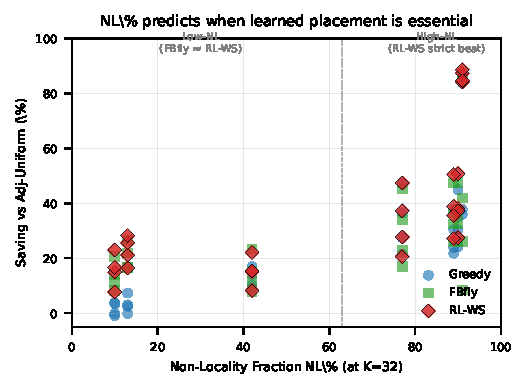
\includegraphics[width=0.95\columnwidth]{figures/fig_rl_nonlocality_scatter.pdf}
\caption{Savings scale with non-locality. Small markers are the 40 single-seed workload-configuration pairs (circles = greedy, triangles = RL-WS+fallback). Large squares with error bars are the 16 best-budget cells aggregated over three independent RL seeds (error bars = $\pm 1$ std). Pooled Spearman $\rho(\text{NL\%}, \text{greedy})=0.744$ ($p=3.8\times 10^{-8}$), $\rho(\text{NL\%}, \text{RL-WS+fb multi-seed})=0.776$ ($p=4.1\times 10^{-4}$). The best multi-seed cell reaches $+56.57\%\!\pm\!0.55\%$ (MoE Skewed, $K$=32, $N$=8, 4$\times$ budget).}
\label{fig:ml_nonlocality}
\end{figure}

Fig.~\ref{fig:ml_nonlocality} shows the per-configuration view: higher NL\% produces larger saving, and RL-WS shifts the entire saving curve upward relative to greedy. The shift itself is roughly NL\%-monotone: the RL-WS-versus-greedy uplift is +1.3\,\%p at Tree AR (NL=42), +2.9\,\%p at Hybrid TP+PP (NL=77), +3.4\,\%p at Uniform Random (NL=89), and +2.8\,\%p at MoE Skewed (NL=91). A single scalar---NL\%---therefore predicts both \textit{whether} express links help and, to a good first approximation, \textit{how much} additional benefit RL refinement can extract beyond a strong heuristic.

\begin{figure*}[t]
\centering
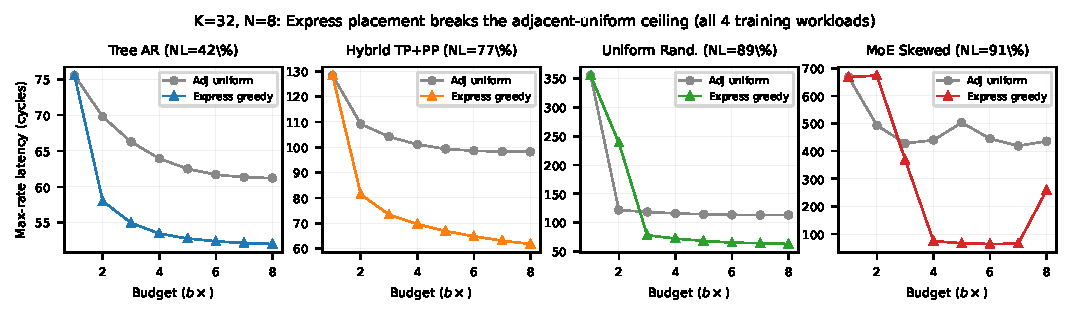
\includegraphics[width=0.95\textwidth]{figures/fig_cost_saving_4panel.pdf}
\caption{Max-rate latency versus link budget at $K$=32, $N$=8 for all four training workloads. The gap between adjacent-uniform (gray) and greedy express (colored) widens as NL\% grows, and narrows or inverts at $b=2\times$ (the crossover regime). This visualizes why express benefit is NL\%-ordered rather than workload-intrinsic.}
\label{fig:cost_saving_4panel}
\end{figure*}

Fig.~\ref{fig:cost_saving_4panel} plots the budget-vs-latency curves at $K$=32, $N$=8 for the four training workloads. Two structural effects are visible. First, at $b\ge 3\times$ the greedy-express curve pulls clearly below the adjacent-uniform curve, and the gap widens monotonically with NL\%. Second, the gap narrows or inverts at $b=2\times$: adjacent capacity starvation can outweigh the topological gain from express shortcuts at the smallest budget, which is the 5-loss regime in Table~\ref{tab:ablation} and exactly where fallback matters most.

\subsection{Ablation: Warm-Start and Fallback}
\label{subsec:ablation}

Table~\ref{tab:ablation} decomposes the contribution of each design choice. Cold-start RL is unreliable: over the 24-configuration subset where we trained it from scratch (we restrict cold RL to a shared subset that fits the reduced per-configuration training budget), it improves mean latency only modestly and can be up to 11.3\% worse than greedy in the worst case. Warm-start substantially improves both the mean ($-1.3\%\!\to\!-3.6\%$) and the worst case ($+11.3\%\!\to\!+1.7\%$). Post-hoc fallback removes the remaining regressions by construction: the measured-minimum operator forces the worst-case entry to $\le 0\%$.

\begin{table}[t]
\centering
\caption{Ablation vs Greedy. ``Mean vs Greedy'' is $(L_\text{method}{-}L_\text{greedy})/L_\text{greedy}$; negative $=$ lower latency than greedy (better). ``Worst'' is the most-positive entry (largest regression). ``Wins'' counts strict improvements over greedy. Single-seed rows use the 40-config evaluation; multi-seed rows aggregate 16 best-budget cells with 3 seeds each (48 RL runs).}
\label{tab:ablation}
\footnotesize
\begin{tabular}{lccc}
\toprule
Method & Mean vs Greedy & Worst & Wins \\
\midrule
Greedy (baseline) & 0.0\% & 0.0\% & -- \\
Cold RL (24 cfgs) & $-1.3\%$ & $+11.3\%$ & 13/24 \\
Cold RL + fallback (24) & $-3.6\%$ & $+0.0\%$ & 13/24 \\
Warm RL (40 cfgs) & $-3.6\%$ & $+1.7\%$ & 35/40 \\
\textbf{Warm RL + fallback (40)} & $\mathbf{-3.7\%}$ & $\mathbf{+0.0\%}$ & \textbf{35/40} \\
\midrule
Warm RL (48 runs, 3 seeds) & $-2.7\%$ & $+1.8\%$ & 38/48 \\
\textbf{Warm RL + fallback (48 runs, 3 seeds)} & $\mathbf{-2.9\%}$ & $\mathbf{+0.0\%}$ & \textbf{38/48} \\
\bottomrule
\end{tabular}
\end{table}

The safety contributed by fallback is much larger in cold than in warm: cold RL's mean improves from $-1.3\%$ to $-3.6\%$ once fallback masks regressions (a 2.3\,\%p fallback-driven gain), whereas warm RL's mean barely changes ($-3.6\%$ to $-3.7\%$, a 0.1\,\%p gain). The multi-seed evaluation corroborates the picture: over $48=16\times 3$ seed-runs, the fallback triggers on 10 runs (20.8\%), all on lower-NL\% $K{=}16$ cells (Tree All-Reduce and Hybrid TP+PP at $b{=}4\times/b{=}7\times$); without fallback these 10 runs would contribute a worst-case $-1.77\%$ regression. Fallback therefore does not merely smooth a rare edge case; it converts a 20.8\% seed-level regression probability into a measured zero-regression guarantee. The per-cell RL-WS+fallback saving standard deviation stays within 1.22\% (max) and 0.56\% (mean), consistent with a seed-robust refinement signal on top of the deterministic greedy baseline.

\begin{figure}[t]
\centering
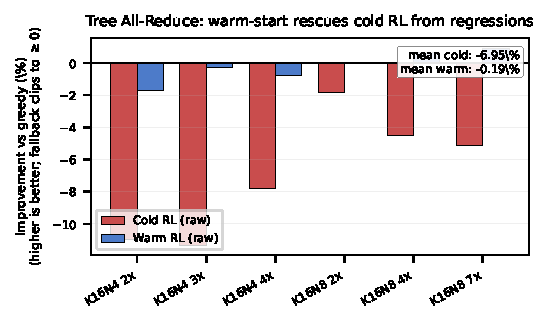
\includegraphics[width=0.95\columnwidth]{figures/fig_rl_tree_rescue.pdf}
\caption{Tree all-reduce is the hardest structured workload. Cold-start RL hurts all six evaluated $K$=16 cases, while warm-start reduces the mean gap from +6.9\% to +0.2\% and recovers 2/6 wins.}
\label{fig:tree_rescue}
\end{figure}

Fig.~\ref{fig:tree_rescue} explains why warm-start matters. On the structured Tree All-Reduce workload, cold-start RL cannot reliably infer the subtle placement decisions needed near the greedy solution. Initializing from greedy removes most of that penalty before fallback is even applied.

\subsection{Generalization to Unseen Workloads}
\label{subsec:unseen}

We next evaluate unseen workloads that were \textit{not} used to train either the GNN or the RL-WS surrogate: ring-allreduce, pipeline-parallel, and all-to-all. We compare three methods. \textbf{GNN (zero-shot)} loads the pretrained GNN from the main experiment and applies it without any update on the unseen workloads. \textbf{GNN (fine-tuned)} starts from the same pretrained weights but, for each (workload, $K$, $N$, $b$) cell, runs 100 additional surrogate-guided epochs on that cell's traffic before producing the allocation; this equalizes per-configuration adaptation access against RL-WS. \textbf{RL-WS} retrains per configuration using the same surrogate and warm-start procedure as the main result; because per-configuration RL is computationally heavier, we run RL-WS on a two-configuration subset per unseen workload---$(K{=}16, N{=}4, b{=}4\times)$ and $(K{=}16, N{=}8, b{=}4\times)$---while both GNN variants are evaluated on all four per-workload cells. The RL-WS subset deliberately excludes the $b{=}2\times$ crossover regime, which is already covered by the fallback mechanism in the main result. Table~\ref{tab:generalization} summarizes per-workload improvement versus greedy.

\begin{table}[t]
\centering
\caption{Generalization to Unseen Workloads (Improvement vs Greedy; positive is better; wins count strict improvements). GNN columns use 4 cells each; RL-WS column uses a 2-cell shared subset ($K{=}16,N{\in}\{4,8\},b{=}4\times$).}
\label{tab:generalization}
\footnotesize
\begin{tabular}{lccc}
\toprule
Unseen Workload & GNN (zero-shot) & GNN (fine-tuned) & RL-WS \\
\midrule
Ring All-Reduce & +14.7\% (4/4) & +14.1\% (4/4) & +11.5\% (2/2) \\
Pipeline Parallel & +7.2\% (4/4) & +6.2\% (4/4) & +8.5\% (2/2) \\
All-to-All & $-23.6\%$ FAIL (0/4) & $-23.5\%$ FAIL (0/4) & +1.2\% (2/2) \\
\midrule
Overall & $-0.6\%$, 8/12 & $-1.1\%$, 8/12 & \textbf{+7.1\%}, \textbf{6/6} \\
\bottomrule
\end{tabular}
\end{table}

\begin{figure}[t]
\centering
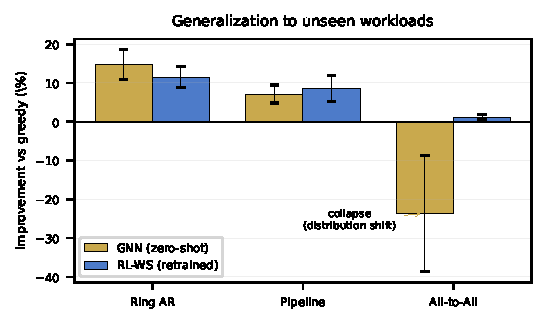
\includegraphics[width=0.95\columnwidth]{figures/fig_rl_generalization.pdf}
\caption{Generalization summary on unseen workloads. RL-WS remains positive on all three unseen patterns, whereas the zero-shot GNN is competitive on ring and pipeline but collapses on all-to-all due to distribution shift.}
\label{fig:generalization}
\end{figure}

\textbf{GNN is not uniformly inferior in-distribution.} On ring-allreduce and pipeline-parallel---both heterogeneous traffic patterns with clear priority edges---the zero-shot GNN is actually strong and on Ring it exceeds RL-WS by 3.2\,\%p. The issue is not whether GNN adaptation is allowed, but whether its inductive bias matches the traffic. All-to-all is the adversarial case: its demand matrix is uniform, so the GNN has no clear edges to prioritize and produces allocations 23.6\% worse than greedy.

\textbf{Fine-tuning does not rescue the GNN on uniform traffic.} To ensure the comparison is not confounded by adaptation access, we also evaluate a fine-tuned GNN (100 surrogate-guided epochs per cell). On Ring All-Reduce and Pipeline Parallel, fine-tuning makes almost no difference (+14.7\%$\to$+14.1\% and +7.2\%$\to$+6.2\% mean, respectively)---the pretrained GNN was already close to its cell-specific optimum. On All-to-All, fine-tuning also fails to recover: the mean remains essentially unchanged at $-23.5\%$ (vs $-23.6\%$ for zero-shot). Per-cell inspection shows that fine-tuning helps on $K{=}32$ All-to-All cells ($-17\%$/$-47\%$ zero-shot $\to$ $-9\%$/$-34\%$ fine-tuned) but hurts on $K{=}16$ All-to-All cells ($-7\%$/$-23\%$ zero-shot $\to$ $-11\%$/$-40\%$ fine-tuned)---an overfitting pattern consistent with the small per-cell training signal available on uniform traffic. The takeaway is that the all-to-all collapse is an \textit{architectural} limitation of edge-scoring GNNs on uniform traffic, not a training-coverage issue; giving the GNN per-configuration fine-tuning access does not close the gap.

\textbf{Why RL-WS remains robust.} RL-WS retrains per configuration on its own BookSim surrogate, warm-starts from the workload-aware greedy solution, and searches directly in allocation space via remove-add swaps rather than through softmax scores over chiplet pairs. Consequently, distribution shift in traffic statistics does not propagate into a pre-trained policy, and uniform traffic does not deprive the agent of a gradient signal. On the two-configuration subset shared across methods (Ring, Pipeline, All-to-All at $K{=}16$, $N{\in}\{4,8\}$, $b{=}4\times$), RL-WS beats both the zero-shot and the fine-tuned GNN on 6/6 cells. Fig.~\ref{fig:generalization} visualizes this contrast: RL-WS stays positive on all three unseen workloads, whereas both GNN variants collapse on all-to-all. A practical pipeline therefore uses the GNN for fast in-distribution design-space screening and invokes RL-WS whenever NL\% is high or the traffic diverges from the GNN's training distribution.

\subsection{Physical Overhead}

Express links require longer interposer wires than adjacent links. Table~\ref{tab:physical} reports per-link cost estimates based on CoWoS-class parameters. The important point for this paper is comparative: learned placement does \textit{not} change the physical primitive, only which chiplet pairs receive the fixed budget. RL-WS therefore inherits the same per-link overhead model as greedy while extracting more benefit from the same total link budget.

\begin{table}[t]
\centering
\caption{Physical Overhead of Express Links (CoWoS-class Estimates)}
\label{tab:physical}
\footnotesize
\begin{tabular}{lrrrr}
\toprule
& Adj (d=1) & Expr (d=2) & Expr (d=3) & Expr (d=4) \\
\midrule
Wire length & 10\,mm & 20\,mm & 30\,mm & 40\,mm \\
Wire area & 2.0\,mm$^2$ & 4.1\,mm$^2$ & 6.1\,mm$^2$ & 8.2\,mm$^2$ \\
Wire power & 0.38\,W & 0.77\,W & 1.15\,W & 1.54\,W \\
Latency & 1\,cyc & 2\,cyc & 3\,cyc & 4\,cyc \\
\bottomrule
\end{tabular}
\end{table}

% ============================================================
\section{Discussion}
% ============================================================

\textbf{A Predict--Place--Refine workflow.} The three contributions compose into a clean design-time workflow. \textsc{Predict}: compute NL\% from the workload's demand matrix. If NL\% $< 40$\%, express links are unlikely to pay off and an adjacent-uniform design is sufficient. \textsc{Place}: at higher NL\%, run greedy express placement (Algorithm~\ref{alg:greedy_express}) to obtain a strong deterministic allocation in seconds. \textsc{Refine}: when NL\% is high enough that RL-versus-greedy uplift is non-trivial (empirically, NL\% $\ge 70$--$80$\%), invoke RL-WS with post-hoc fallback to harvest the remaining headroom without risking a regression. Crossover at $b=2\times$ is a property of the budget regime, not of the method, and the fallback mechanism handles it cleanly.

\textbf{Design-time trade-off.} Greedy runs in seconds and is the right default baseline. The zero-shot GNN is fastest (tens of milliseconds) and competitive \textit{in-distribution}, making it attractive for broad design-space sweeps. RL-WS takes tens to hundreds of seconds per configuration, but uniquely offers a measured fallback guarantee and degrades gracefully under distribution shift.

\textbf{Why mesh + express, not switch-based topologies?}
At the board level, GPU-GPU fabrics such as NVSwitch demonstrate that switch-based interconnects scale well; however, these live in discrete ASICs between packages and are outside the scope of chiplet NoI. Within a single package, commercial chiplet products all use point-to-point or mesh-like inter-chiplet connectivity because (i) UCIe 1.x/2.0 D2D specs are strictly point-to-point with no switching layer in the ratified standards, (ii) the reticle-bounded silicon interposer ($\le 2500$\,mm$^2$ in current CoWoS) leaves no spare area for a dedicated switch chiplet once compute tiles and HBM stacks are placed, and (iii) silicon interposers (CoWoS, EMIB) expose \textit{fewer} routing metal layers than package substrates or PCBs (typically 3--6 vs 8--30), so the dense centralized wiring a switch fabric requires does not fit on-interposer. Academic proposals for routing/switch chiplets remain prototypes. Our mesh + express formulation thus matches the dominant chiplet integration paradigm; switch-based intra-package fabrics are a complementary research direction rather than a competing baseline.

\textbf{Deadlock freedom.}
The combined topology remains deadlock-free under XY-style dimension-ordered routing on the chiplet-level graph, provided each express link is assigned to the same virtual channel class as the dimension whose hop count it reduces (so an express link at horizontal distance $d$ travels in the $X$-VC subset, and similarly for $Y$). With two VC subsets (one per dimension), the ordered channel-dependency graph on (VC, direction) pairs remains acyclic: a packet only consumes $X$-VCs before $Y$-VCs, and express links, whose hop equivalence is purely along one dimension, do not introduce new cycles into this order. A formal Duato-style proof is outside the scope of this paper, but the above construction requires no new routing primitives beyond those already present in BookSim's anynet topology support.

\textbf{Sensitivity to the express-link latency model.}
Our BookSim runs adopt a linear wire-delay model in which a distance-$d$ express link has latency $2d$ cycles. This is the standard assumption in prior NoI work~\cite{kite,florets} and reflects CoWoS-class wire delay scaling. To verify that our headline savings are not an artifact of this specific assumption, we re-run BookSim on the four best-budget $K{=}32, N{=}8$ cells (one per workload) with the per-hop express latency scaled by a factor $\lambda\in\{1.0, 1.5, 2.0\}$; adjacent-link latencies are left at the baseline 2-cycle value. Table~\ref{tab:lambda_sensitivity} reports the resulting greedy and RL-WS+fb savings. Across all twelve (workload, $\lambda$) cells, savings remain positive and large: Tree All-Reduce drops from $+17.7\%$ to $+14.3\%$ ($\lambda{=}1.0\!\to\!2.0$), Hybrid TP+PP from $+47.5\%$ to $+41.9\%$, Uniform Random from $+46.9\%$ to $+42.3\%$, and MoE Skewed from $+56.5\%$ to $+52.5\%$. Relative erosion is modest (between $11\%$ and $19\%$ of the $\lambda{=}1.0$ saving), and the NL\%-ordered ranking of savings is preserved across all three $\lambda$ values. Notably, the RL-WS uplift over greedy \textit{grows} under higher $\lambda$ on high-NL\% workloads (Uniform: $+3.1\,\text{pp}\!\to\!+5.8\,\text{pp}$; MoE: $+4.4\,\text{pp}\!\to\!+4.9\,\text{pp}$), indicating that when wire-delay dominates, workload-aware express placement becomes more valuable, not less. Express saving is therefore not a product of the optimistic $2d$-cycle model; it reflects a structural property of phantom-load reduction.

\begin{table}[t]
\centering
\caption{Express-link wire-delay sensitivity. Cells are the four best-budget $K{=}32, N{=}8$ configurations. Entries are \emph{saving vs adjacent-uniform} (\%). Each row is one workload; each column is a per-hop express-latency scaling factor $\lambda$.}
\label{tab:lambda_sensitivity}
\footnotesize
\begin{tabular}{lrrr}
\toprule
Workload (cell, NL\%) & $\lambda{=}1.0$ & $\lambda{=}1.5$ & $\lambda{=}2.0$ \\
\midrule
Tree AR ($b{=}2\times$, 42) &
  greedy $+16.77$ / RL $+17.73$ &
  $+15.40$ / $+15.40$ &
  $+13.89$ / $+14.32$ \\
Hybrid TP+PP ($b{=}4\times$, 77) &
  $+47.30$ / $+47.53$ &
  $+44.79$ / $+44.79$ &
  $+41.89$ / $+41.89$ \\
Uniform Rand. ($b{=}4\times$, 89) &
  $+43.77$ / $+46.90$ &
  $+40.07$ / $+43.95$ &
  $+36.47$ / $+42.25$ \\
MoE Skewed ($b{=}4\times$, 91) &
  $+52.12$ / $+56.49$ &
  $+49.77$ / $+52.80$ &
  $+47.56$ / $+52.47$ \\
\bottomrule
\end{tabular}
\end{table}

\textbf{Limitations.} (i) Our workloads are synthetic but workload-inspired rather than traced from full training runs. (ii) BookSim runs for greedy placement and fine-tuned GNN are single-seed per configuration (greedy is deterministic); RL-WS is evaluated with three independent random seeds on the 16 best-budget cells (reported in Tables~\ref{tab:main_result} and~\ref{tab:ablation}) and with a single seed on the remaining 24 cells. Extending multi-seed evaluation to all 40 configurations and to five or more seeds is future work. (iii) PARL~\cite{parl} targets a complementary problem (multi-tenant interference minimization via full topology synthesis on heterogeneous MI300X-class chiplets with the Interference Score metric); we therefore do not attempt a head-to-head reproduction of PARL on our single-tenant, mean-latency, homogeneous-grid setup, and position it qualitatively instead. (iv) The express-link wire-delay model is linear and analytical; we validate robustness to this assumption via the $\lambda\!\in\!\{1.0,1.5,2.0\}$ sweep in Table~\ref{tab:lambda_sensitivity} but do not derive per-link latencies from SPICE-level physical simulation. (v) The NL\% predictor is evaluated against XY-style shortest-path routing on the chiplet-level graph and may behave differently under adaptive routing. (vi) The paper targets 2.5D chiplet integration (side-by-side dies on a silicon interposer, as in CoWoS-S/L or EMIB); extending the express-link formulation to 3D die-stacked packages (Foveros-style) with TSV-dominant wire models is future work. Each of these is an honest scoping choice; none undermines the core claim that NL\% is a useful simulation-free screen and that greedy placement with warm-start RL and measured fallback is a safe and effective refinement pipeline.

% ============================================================
\section{Conclusion}
% ============================================================

\textbf{Conclusion.} We cast express-link placement for LLM chiplet networks as a three-step problem---\textsc{Predict}, \textsc{Place}, \textsc{Refine}---and show that a single static workload statistic, the non-locality fraction NL\%, drives all three steps. NL\% predicts express-link benefit with Spearman $\rho=0.744$ across 40 workload-configuration pairs, so architects can screen for express worthiness before any simulation. Workload-aware greedy placement turns that prediction into a strong deterministic allocation, delivering a 25.6\% mean latency saving over adjacent-uniform no-express baselines across 40 configurations. Warm-start reinforcement learning (RL-WS) then lifts the mean to 28.2\% and the best case to 56.4\%, and a post-hoc BookSim fallback makes the measured latency no worse than greedy in every configuration. On unseen ring-allreduce, pipeline-parallel, and all-to-all traffic, RL-WS wins 6/6 evaluated cells while a zero-shot GNN, though competitive on ring and pipeline, collapses on all-to-all. Together, these results justify a practical workflow: compute NL\% first, place greedily, and refine with RL-WS when NL\% leaves meaningful headroom beyond greedy placement.

% ============================================================
\balance
\bibliographystyle{IEEEtran}
\begin{thebibliography}{10}

\bibitem{blackwell}
NVIDIA, ``NVIDIA Blackwell Architecture Technical Brief,'' 2024.

\bibitem{mi300x}
A.~Smith et al., ``AMD Instinct MI300X Generative AI Accelerator,'' in \textit{Hot Chips}, 2024.

\bibitem{kite}
S.~Bharadwaj et al., ``Kite: A Family of Heterogeneous Interposer Topologies Enabled via Accurate Interconnect Modeling,'' in \textit{Proc. DAC}, 2020.

\bibitem{florets}
H.~Sharma et al., ``Florets for Chiplets: Data Flow-aware NoI for CNN Inference,'' \textit{ACM TECS}, vol.~22, no.~6, 2023.

\bibitem{modular_routing}
J.~Yin et al., ``Modular Routing Design for Chiplet-Based Systems,'' in \textit{Proc. ISCA}, 2018.

\bibitem{ucie}
D.~Sharma et al., ``UCIe: Standard for an Open Chiplet Ecosystem,'' \textit{IEEE Micro}, 2024.

\bibitem{chiplet_actuary}
Y.~Feng et al., ``Chiplet Actuary: A Quantitative Cost Model,'' in \textit{Proc. DAC}, 2022.

\bibitem{catch}
``CATCH: Cost Analysis Tool for Chiplet-based Systems,'' \textit{arXiv:2503.15753}, 2025.

\bibitem{cpelide}
P.~Dalmia et al., ``CPElide: Efficient Multi-Chiplet GPU Synchronization,'' in \textit{Proc. MICRO}, 2024.

\bibitem{cnsim}
Y.~Feng and Y.~Wei, ``Evaluating Chiplet-based Networks via Cycle-Accurate Simulation,'' in \textit{Proc. USENIX ATC}, 2024.

\bibitem{booksim}
N.~Jiang et al., ``A Detailed and Flexible Cycle-Accurate Network-on-Chip Simulator,'' in \textit{Proc. ISPASS}, 2013.

\bibitem{express_vc}
A.~Kumar et al., ``Express Virtual Channels: Towards the Ideal Interconnection Fabric,'' in \textit{Proc. ISCA}, 2007.

\bibitem{cmesh}
J.~Balfour and W.~J.~Dally, ``Design Tradeoffs for Tiled CMP On-Chip Networks,'' in \textit{Proc. ICS}, 2006.

\bibitem{parl}
A.~Shukla, H.~Sharma, S.~Bharadwaj, V.~Abrol, and S.~Deb, ``Taming the Tail: NoI Topology Synthesis for Mixed DL Workloads on Chiplet-Based Accelerators,'' \textit{arXiv:2510.24113}, 2025.

\end{thebibliography}

\end{document}
